\chapter{Gérer les lectures}
\section{Sélectionner un poisson}
Le menu \textit{Lectures} permet d'accéder à une fenêtre de recherche des poissons. 

\begin{figure}[H]
\centering
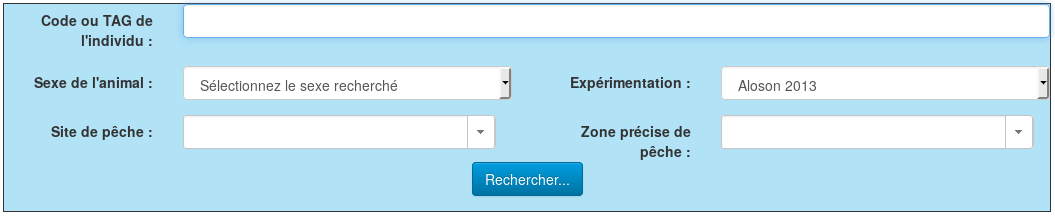
\includegraphics[width=\linewidth]{images/recherchePoisson}
\caption{Fenêtre de recherche des poissons}
\end{figure}

Seules les expérimentations pour lequel l'utilisateur dispose des droits de lecture sont affichées. Il est possible de rechercher les poissons en utilisant un des deux codes disponibles (code de l'individu ou TAG).

La sélection d'un poisson permet d'atteindre sa page de détail :
\begin{figure}[H]
\centering
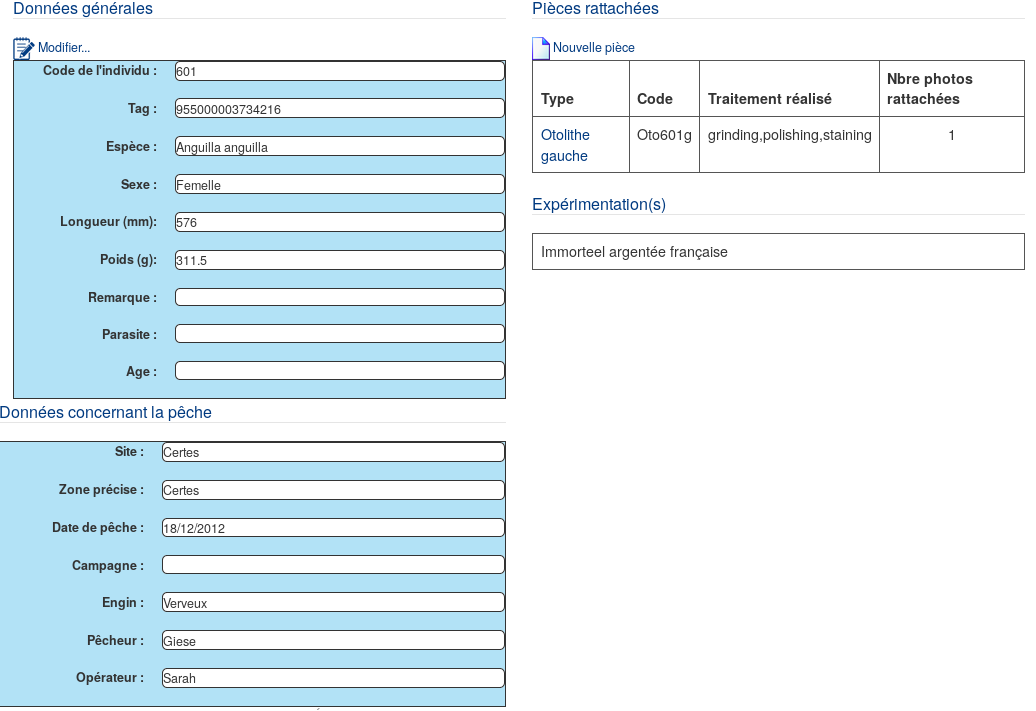
\includegraphics[width=\linewidth]{images/poissonDetail}
\caption{Fenêtre de détail d'un poisson}
\end{figure}

\subsection{Modifier un poisson}

Si les droits sont suffisants, l'utilisateur peut modifier les informations concernant un poisson. 

\begin{figure}[H]
\centering
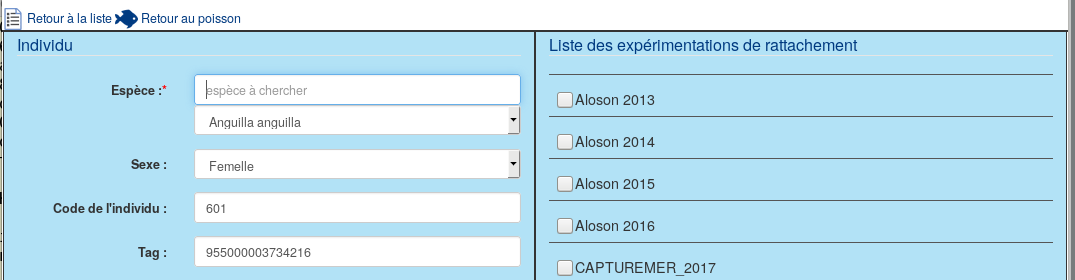
\includegraphics[width=\linewidth]{images/poissonModif}
\caption{Fenêtre de modification d'un poisson}
\end{figure}

La sélection de l'espèce se fait en tapant quelques caractères de l'espèces à chercher (nom latin ou français), puis en sélectionnant dans la liste déroulant l'information pertinente.

À noter que cet écran permet de l'associer avec une ou plusieurs expérimentations (au moins une à sélectionner -- ne pas supprimer l'expérimentation initiale sous peine de \og perdre \fg{} le poisson et de ne pas pouvoir le retrouver par l'application).

\subsection{Ajouter des pièces calcifiées}

Si elles n'ont pas été créées lors de l'importation, les pièces calcifiées peuvent être rajoutées manuellement. Seul le type de la pièce est obligatoire.

\section{Gestion des photos}

L'ajout d'une photo n'est possible que depuis le détail d'une pièce calcifiée. Il est possible d'en ajouter autant que nécessaire pour la même pièce, mais la lecture n'est réalisable que photo par photo.

\subsection{Limitations quant au format et aux dimensions d'une photo}

Si le format TIFF est souvent plébiscité pour son absence de perte d'informations, il présente l'inconvénient de ne pas être supporté par les navigateurs et ne peut pas être utilisé pour réaliser les lectures. De plus, il est assez gourmand en espace de stockage.

Le logiciel autorise toutefois l'importation de photos au format TIFF, sachant que celles-ci seront transformées en JPG au moment de la lecture (le format d'origine est conservé dans la base de données).

Les logiciels associés aux microscopes peuvent générer des photos au format TIFF mal formées (messages d'erreur lors de leur ouverture). Si une photo n'arrive pas à être importée, il convient de l'ouvrir avec le logiciel GIMP \cite{gimp}, puis l'enregistrer de nouveau : les messages d'erreur seront supprimés lors de cette étape. Ce logiciel est également très efficace pour réduire la taille d'une photo trop volumineuse.

Pour des raisons de performance, il est déconseillé d'importer des photos de plus de 50 Mo, celles-ci étant retraitées par le serveur avant d'être stockées.

Les photos sont stockées dans la base de données dans leur format original et sous forme de miniature, pour réduire les temps de traitement.

\subsection{Repère de mesure et longueur de référence}

Il est courant d'insérer un repère de mesure sur une photo. En connaissant sa longueur en pixels (dans la photo d'origine), il est alors facile de calculer des distances sur la photo, et notamment les écartements entre les points lors de la lecture.

Si ces deux informations sont renseignées, les lecteurs n'auront pas besoin de mesurer individuellement la taille de la longueur de référence pour recalculer les dimensions mesurées sur la photo.

\section{Gestion des lectures}

Il est possible de réaliser autant de lectures que nécessaire, celles-ci étant datées.

Pour des questions de performances, la taille de la photo transmise au navigateur peut volontairement être réduite. Les résolutions par défaut proposées sont les suivantes :
\begin{itemize}
\item 800x600
\item 1024x768
\item 1280x1024
\item 1600x1300
\item taille originale
\end{itemize}

Les lecteurs peuvent choisir la résolution qui leur convient le mieux, sachant que plus la photo est détaillée, plus elle est volumineuse. 

Le placement des points sur la photo est recalculé en tenant compte du facteur de réduction : le logiciel permet ainsi de visualiser l'ensemble des lectures effectuées quelle que soit la résolution utilisée par chaque lecteur.

\subsection{Tableau des lectures}

\begin{figure}[H]
\centering
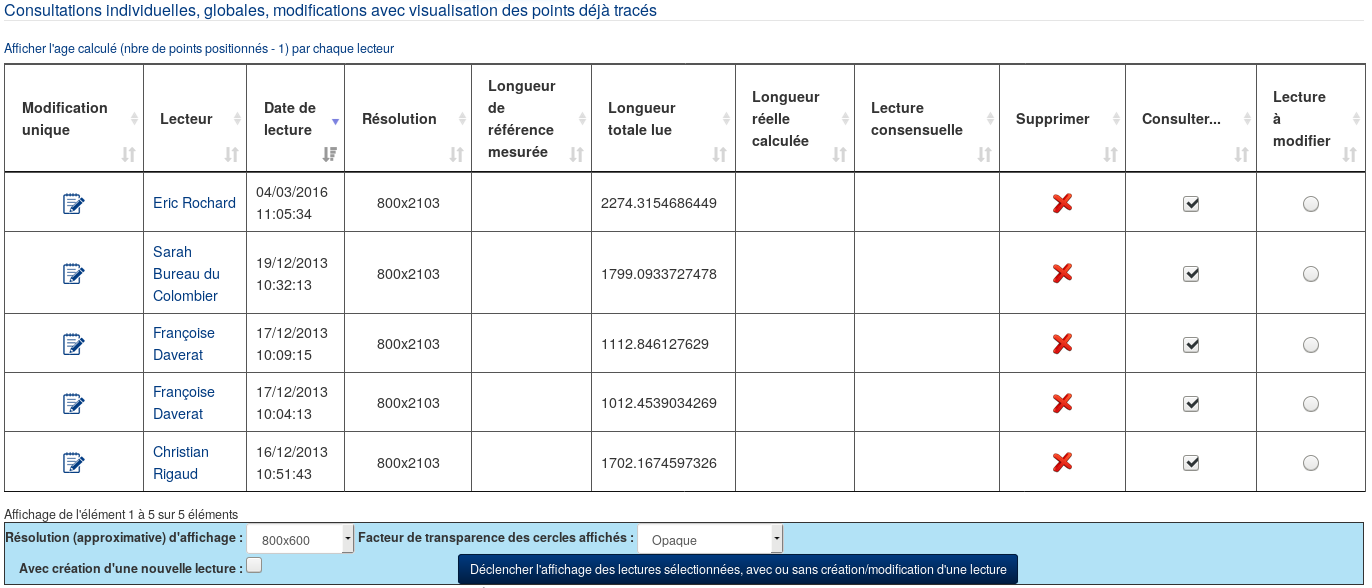
\includegraphics[width=\linewidth]{images/lectureTableau}
\caption{Tableau récapitulatif des lectures réalisés sur une photo}
\end{figure}

Le tableau des lectures permet de consulter l'ensemble des lectures réalisées, soit individuellement, soit globalement. Le formulaire en bas de tableau permet ainsi de créer une nouvelle lecture en affichant celles qui sont sélectionnées, par exemple pour créer une lecture consensuelle.

Par défaut, pour ne pas influencer les lecteurs, le nombre de segments déterminés par les lecteurs précédents n'est pas affiché. Il suffit de cliquer sur le lien \textit{Afficher l'age calculé (nbre de points positionnés - 1) par chaque lecteur} pour obtenir le nombre de segments identifiés.

Pour faciliter la visualisation des points sur les photos, il est possible d'ajuster leur facteur de transparence, depuis opaque jusqu'à totalement transparent.

\subsection{Réaliser une lecture}

L'écran est organisé en plusieurs parties. Le haut affiche la photo, où pourront être placés les points. Sous la photo, un formulaire permet de modifier le comportement de la lecture ou de préciser des informations complémentaires. Enfin, la page se termine par le tableau des points saisis.

Un clic sur la photo positionne un point, dont les coordonnées seront affichées dans le tableau en bas d'écran. Pour supprimer un point, double-cliquez sur celui-ci.

\subsubsection{Type de lecture}

Le logiciel permet de positionner un premier point (initial) plus grand que les autres, pour identifier une zone centrale correspondant au stade larvaire (par exemple).

Pour cela, positionnez le \textit{type de lecture pour le prochain point} à \textit{Point initial avec cercle élargi}. La taille du cercle sera celle indiquée dans \textit{Rayon (en pixels) du cercle élargi}.

Il est également possible de positionner sur la photo une ligne pour aider à placer les points. Choisissez \textit{Tracé d'une ligne sur la photo (aide à la mesure)}, et placez deux points. Un trait sera affiché sur la photo, et vous pourrez positionner vos points le long de celui-ci (décalage d'un pixel au minimum pour des questions techniques). 
\underline{Attention} : cette ligne n'est pas sauvegardée.

Enfin, si cette information n'a pas été indiquée dans le détail de la photo, le lecteur devra positionner deux points de part et d'autre de la longueur de référence pour pouvoir calculer le plus précisément possible les distances entre chaque point. Pour cela, choisissez l'option \textit{Mesure de la longueur de référence}.

\subsubsection{Numérotation des points}

Les points sont numérotés de 10 en 10. Il est possible d'insérer un point entre deux autres, mais il est alors nécessaire de modifier son numéro pour qu'il s'insère correctement au moment des calculs.

Toutefois, si le premier point saisi est celui au centre de la pièce calcifiée (le point de base), le logiciel peut recalculer automatiquement l'ordre des points en recherchant celui qui est le plus près, sans tenir compte de l'ordre de numérotation. C'est le fonctionnement par défaut.

\subsubsection{Données complémentaires}
Des informations complémentaires peuvent être renseignées :
\begin{itemize}
\item nature de la strie finale : hyaline (ou vitreuse), obscure, ou non déterminée
\item fiabilité de la lecture : 0 pour très incertaine, 0,5 pour incertaine, et 1 pour fiable
\item lecture consensuelle : à renseigner s'il s'agit de la lecture de vérification
\item année de naissance estimée : à partir du nombre de segments et de la date de pêche du poisson (rappelée dans le cartouche en haut d'écran), il est possible de déterminer l'année de naissance
\end{itemize}

\subsubsection{Légende}

Si plusieurs lectures sont affichées, la légende présente les codes de couleur utilisés pour représenter les points positionnés par chaque lecteur, ainsi que les différents paramètres saisis par chacun.

\subsection{Consulter les lectures}

Il est possible de consulter une photo avec les lectures associées, sans pouvoir créer de points. Seules la photo et la légende sont affichées.